% exercise sheet with header on every page for math or close subjects
\documentclass[12pt]{article}
\usepackage{german} 
\usepackage[utf8]{inputenc} 
\usepackage{latexsym} 
\usepackage{multicol}
\usepackage{fancyhdr}
\usepackage{amsfonts} 
\usepackage{amsmath}
\usepackage{amssymb}
\usepackage{enumerate}
\usepackage{MnSymbol}
\usepackage[colorlinks=true,urlcolor=blue]{hyperref}
\usepackage{listings}
\usepackage{graphicx}

% Shortcuts for bb, frak and cal letters
\newcommand{\E}{\mathbb{E}}
\newcommand{\V}{\mathbb{V}}
\renewcommand{\P}{\mathbb{P}}
\newcommand{\N}{\mathbb{N}}
\newcommand{\R}{\mathbb{R}}
\newcommand{\C}{\mathbb{C}}
\newcommand{\Z}{\mathbb{Z}}
\newcommand{\Pfrak}{\mathfrak{P}}
\newcommand{\Pfrac}{\mathfrak{P}}
\newcommand{\Bfrac}{\mathfrak{P}}
\newcommand{\Bfrak}{\mathfrak{B}}
\newcommand{\Fcal}{\mathcal{F}}
\newcommand{\Ycal}{\mathcal{Y}}
\newcommand{\Bcal}{\mathcal{B}}
\newcommand{\Acal}{\mathcal{A}}


% Formatierung
\topmargin -2cm 
\textheight 24cm
\textwidth 16.0 cm 
\oddsidemargin -0.1cm

\setlength{\parindent}{0pt}  % !!!!!!! Hier werden leerzeilen erlaubt ohne dass Latex automatisch einrueckt! !!!!!!! %


%Python code Highlighting
\lstset{language=Python, tabsize=3,
        basicstyle=\ttfamily\small, 
        keywordstyle=\color{keywords},
        commentstyle=\color{comments},
        stringstyle=\color{red},
        showstringspaces=false,
        identifierstyle=\color{green}}

% Code-Highlighting Java
%\lstset{language=Java, breaklines=true, showstringspaces=false}
%\begin{lstlisting}
%    	Hier würde der Java-Code hinkommen und entsprechend die Syntax markiert. Selbst einrücken.
%\end{lstlisting}
%ODER:
% \lstinputlisting[language=Java]{name.py}

\graphicspath{ {images/} }


\begin{document}

% Titel
%\title{\textsc{Hacking}\\ \textsc{Abgabe 0}\\{ \normalsize Gruppe X \hfill Daniel Schäfer (2549458)\\ \hfill Anderer}}
%\maketitle  

% alternativer Titel
\noindent
{\Large \textbf{High-level Computer Vision}} \hfill \textbf{16.05.2016}\\
{\Large \textbf{Exercise 2}} 
\raggedleft \hfill Guillermo Reyes (2556018)\\
\hfill Daniel Schaefer (2549458)\\
\hfill Marc Tonsen(2537359)\\
\hfill Dominik Weber (2548553)\\

\pagenumbering{gobble}
\raggedright


\section*{Code Annotations}




\section*{Question 1: Support Vector MAchines}

\begin{enumerate}[a)]
	\setcounter{enumi}{1}
	\item 	
	Modify the last two parameters of \textbf{get\_train\_dataset\_2d.m} in order to make the classification problem linearly non-separable. Run your visualization for different values of parameter C and comment on its role in the SVM classification algorithm.\\
	
	%\begin{figure}[h]
	%	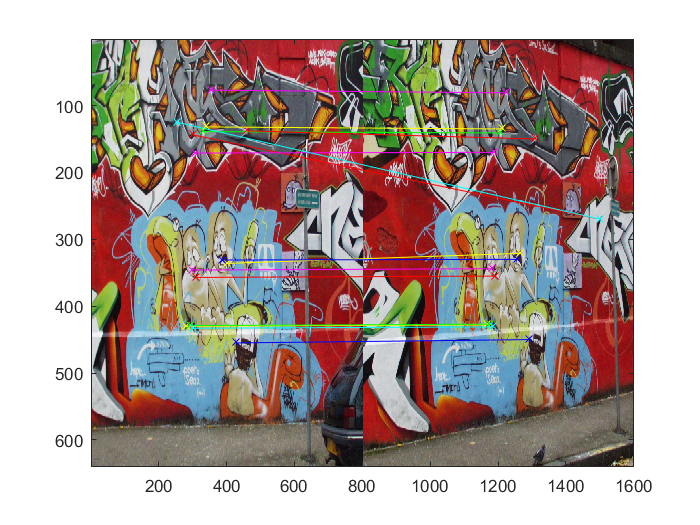
\includegraphics[width=0.5\textwidth]{graf_har_rg}
	%	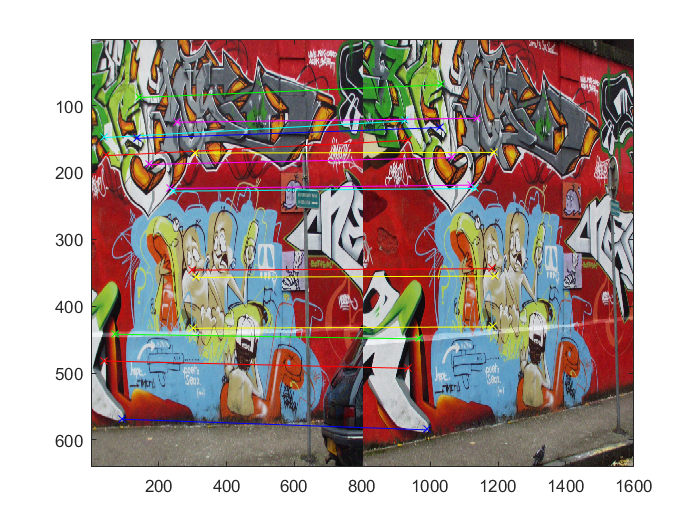
\includegraphics[width=0.5\textwidth]{graf_har_dxdy}
	%	\caption{\textit{Left}: Harris detector with rg histogram descriptor. \textit{Right}: also Harris, but using the dxdy histogram descriptor }
	%\end{figure}

\end{enumerate}

\newpage
\section*{Question 3: Performance Evaluation}
\begin{enumerate}[a)]
	\setcounter{enumi}{1}
	\item 
	Compare the performance of the ystem with and without block normalization step
	\item 
	Compare the performance of the system for cell sizes of 8 and 16 pixels.
	\item
	Write a summary of your observations and submit it along with the corresponding RPC curves
	\item How could you use the system to solve the detection problem in which you are given an image of arbitrary size and the task is to find the position of the people in it?

\end{enumerate}


\end{document}
